%\chapter{Two Resources for Cross-Lingual Phonology and Phonemic Language Modelling}\label{chapter:resources}
\chapter{Two new resources for cross-lingual phonology}\label{chapter:resources}

% Focus is maybe too broad here? Maybe focus more on CHILDES, with phoneme BabyLM as a side-effect.

Phonological research can be enriched by large-scale data-oriented studies that investigate phoneme function across the globe's languages. In this thesis, auto-regressive transformer language models (LMs) are trained using a phoneme-based input representation to gain insights for language model pre-training and distributional phonology. The previous chapter concluded that a suitable training framework is to use developmentally-plausible data, but the majority of language modelling work in this area focuses on orthographic corpora --- requiring a review of whether suitable phonological resources exist to support these experiments.

%This new resource fills several gaps in existing phonemic datasets, which often lack multilingual coverage, spontaneous speech, and a focus on child-directed language.
%There is also a lack of phonemic data for certain domains, preventing phonological research in these areas. In particular, we note that it is difficult to find phonemic data for child-centred speech and, in general, spontaneous speech across several languages.

This chapter begins by reviewing existing phoneme-based datasets in \cref{sec:13-phonemicdatasets}. While written text is plentiful and easily accessible across hundreds of languages, phonemic data is much more limited in availability. In particular, it is difficult to find phonemic data for child-centred speech and, in general, spontaneous speech across several languages. The \emph{de-facto} repository for child-centred data is the Child Language Data Exchange System (CHILDES), as introduced in \cref{sec:12-childes}, but the largely orthographic nature of the data has prevented phonological experimentation.\footnote{CHILDES does contain phonetic transcriptions for some languages as part of the PhonBank project, but only for a select few corpora and only for child-produced utterances, impeding the phonological analysis of child-\emph{directed} speech.} 

\Cref{sec:13-g2p} reviews methods used to create phonemic datasets. Phonemic datasets can be created by employing expert phoneticians to carefully transcribe speech, but this is a time-consuming process and completely infeasible for creating large datasets. Instead, the typical approach is to use tools for grapheme-to-phoneme conversion \citep[G2P;][]{lucassen1984information}. These tools use statistical rules and pronunciation dictionaries to convert orthographic text to a phonemic representation. Open-source G2P tools have been used to create the majority of the phonemic datasets reviewed in \cref{sec:13-phonemicdatasets}. However, the fact that these tools are open-sourced and use a variety of statistical approaches and transcription schemes means that phonemic corpora vary considerably according to their phonemic vocabularies and level of phonetic detail, making it difficult to compare findings and incorporate other linguistic resources into analysis.

\begin{figure}[t]
    \centering
    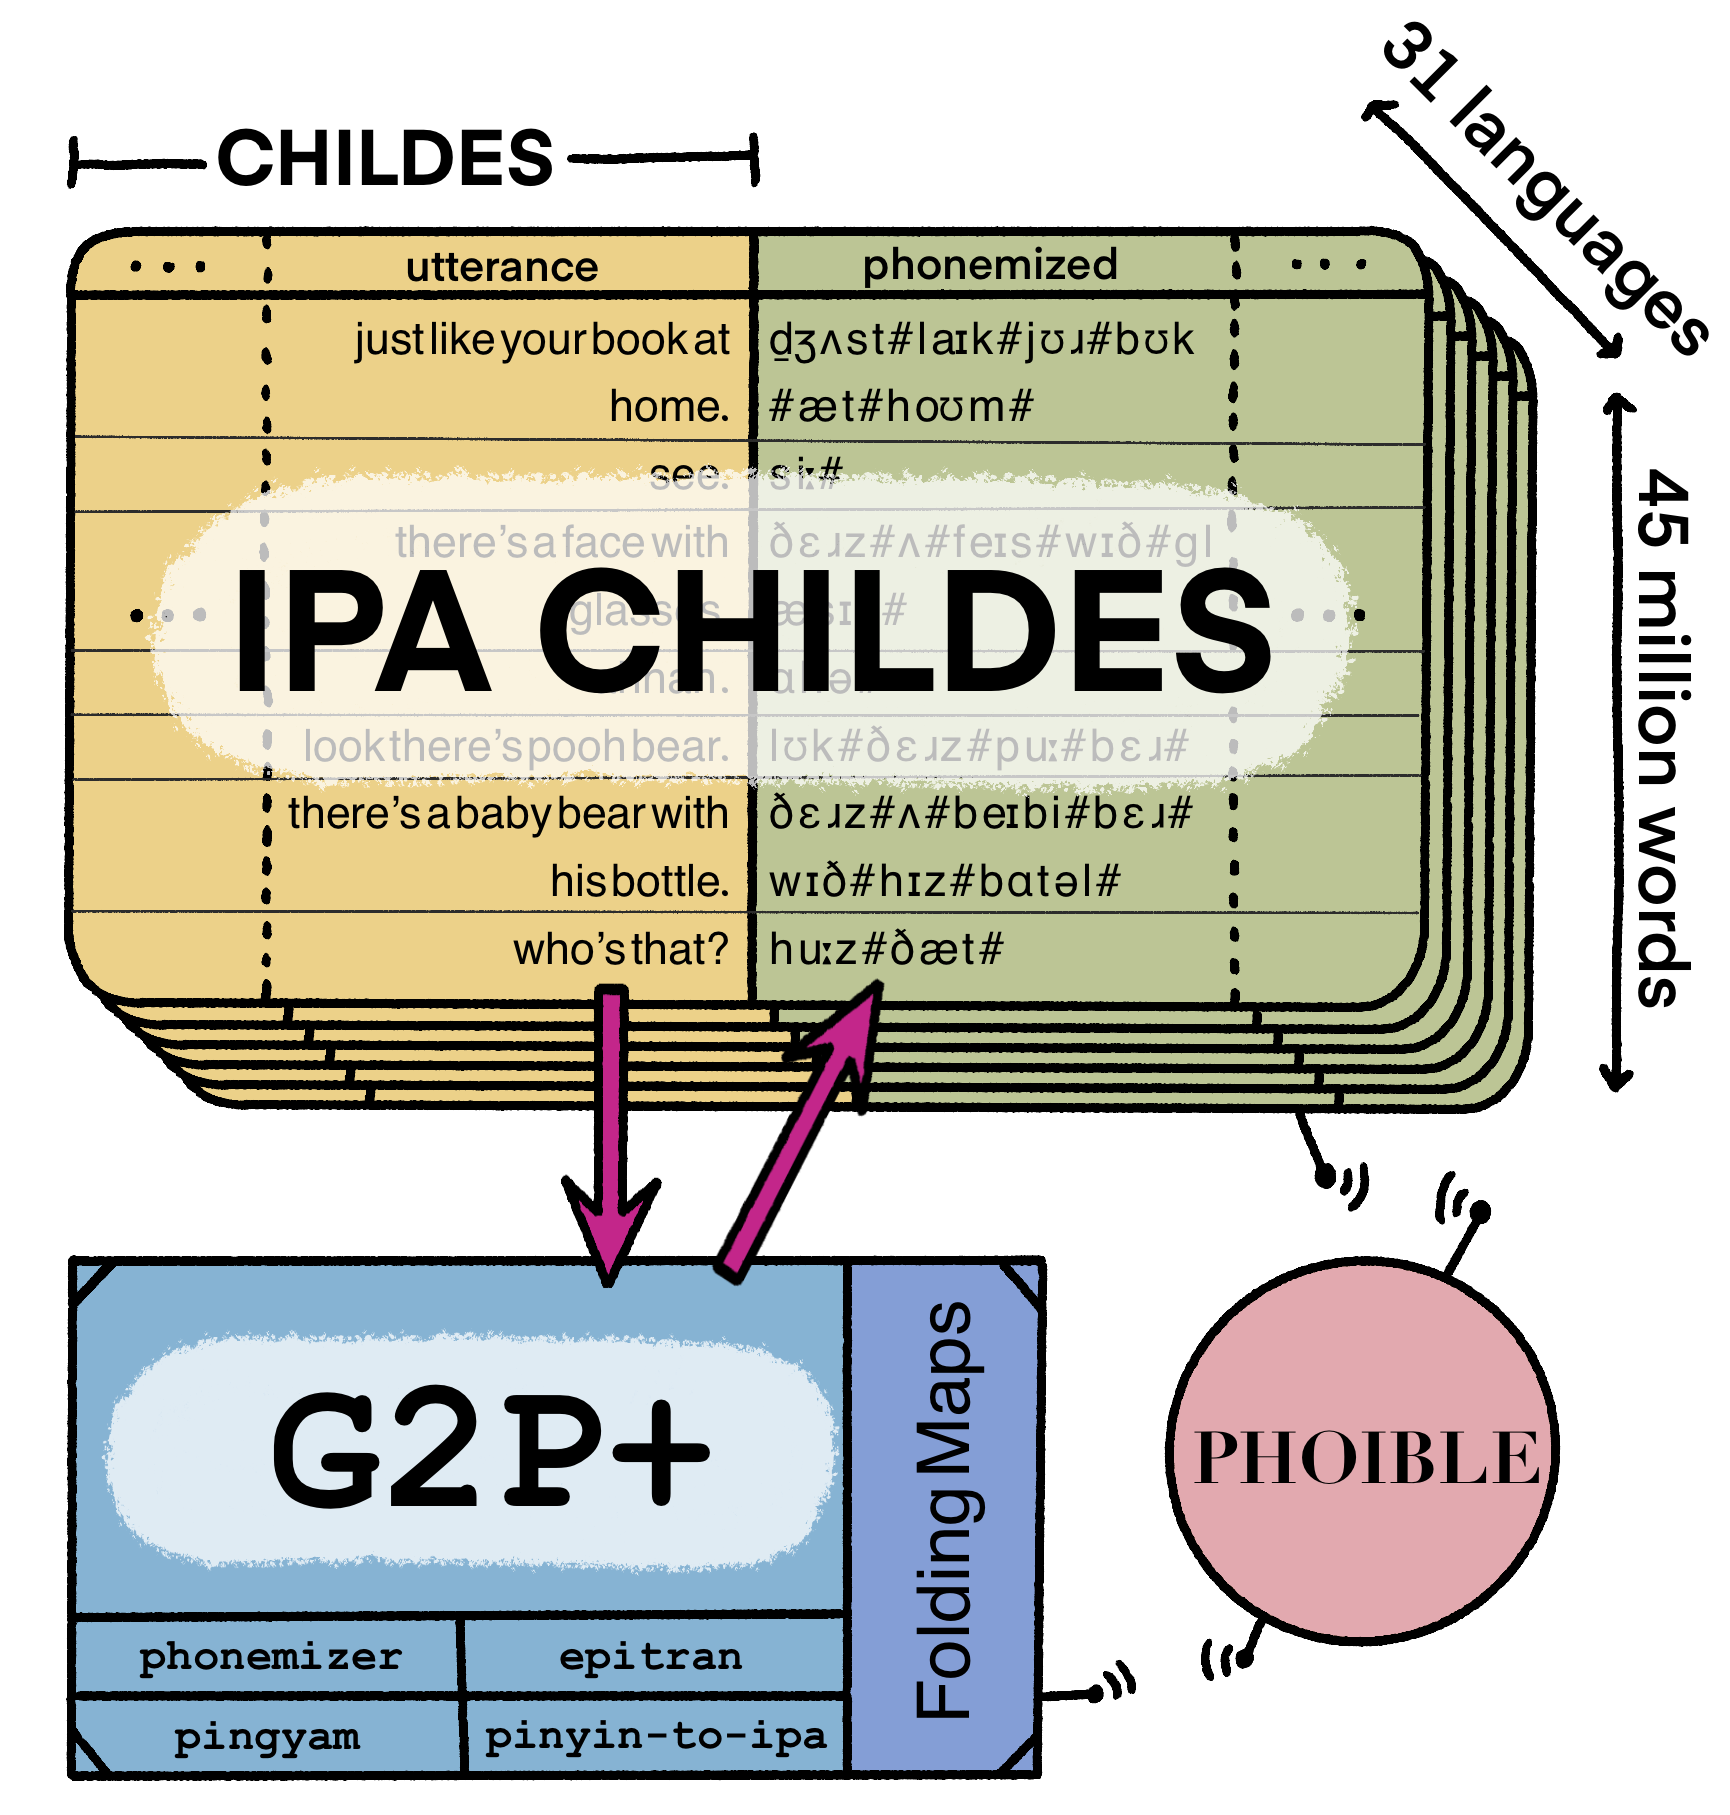
\includegraphics[width=0.5\linewidth]{13Resources/overview.png}
    \caption{An overview of \ipachildes and \gpp, which are introduced in this chapter.}
    \label{fig:13-overview}
\end{figure}

There are thus two major challenges impeding phonological research. First, the lack of consistent G2P conversion, which this chapter addresses by introducing \gpp, a tool for converting orthographic text to a phonemic representation. \gpp leverages existing G2P tools for conversion but carefully maps the output to established phonemic inventories in the \phoible database. Using \phoible inventories not only ensures consistency for each language regardless of the G2P backend used, but the database also contains phonological feature information, supporting fine-grained phonological analysis. Second, to address the lack of a multilingual phonemic dataset of child-centred speech, \gpp is used to convert the majority of the CHILDES database to phonemes. The resulting dataset, \ipachildes, contains phonemic transcriptions of 31 languages in CHILDES, totalling 45 million words. These resources are illustrated in \cref{fig:13-overview}. \ipachildes supports phonological analysis using phoneme LMs, as explored in \cref{chapter:phonology}, and \gpp allows orthographic datasets to be converted to a phonemic representation, used in the modelling study presented in \cref{chapter:modelling}. %Finally, \gpp is also used to convert the BabyLM corpus and evaluation benchmarks to phonemes, to support the technical experiments in \cref{chapter:modelling}.

\section{Phonemic datasets}\label{sec:13-phonemicdatasets}

%Phonemic data is required to investigate a range of linguistic phenomena. Recently, researchers have used data-driven approaches to study morphological theories of acquisition \citep{kirov2018recurrent}, explore the role of distributional information in phonology \citep{mayer-2020-phonology-distribution}, calculate cross-language phonological distance \citep{eden-2018-phonological-distance} and simulate early lexicon learning \citep{goriely2023word}. Despite the benefits of phonemic data, few such datasets exist. 

Phonemic data is required to investigate a range of linguistic phenomena. As introduced in \cref{sec:12-phonemic}, researchers have used data-driven approaches to study morphological theories of acquisition, explore the rule of distributional information in phonology, calculate cross-language phonological distance and simulate early lexicon learning. Despite the benefits of phonemic data, few such datasets exist. 

Written text and audio datasets are far more plentiful than phonemic datasets. Written text, being widely distributed and easy to collect through practices such as web-scraping \citep{bansal-2022-datascaling}, has steered years of NLP research, ranging from the parsers trained on the Penn Treebank \citep{taylor2003penn} to the large language models trained on billion-word datasets like the Pile \citep{pile}. Despite the availability of written text, it is often inappropriate for speech technology and phonological research. Instead, since tape recorders became widely available, researchers have created datasets of human speech. These now include \textbf{elicited} speech corpora such as TIMIT, \citep{garofolo1993darpa}, FLEURS \citep{conneau2023fleurs}, the MSWC \citep{mazumder2021multilingual}, GlobalPhone \citep{schultz2002globalphone} and CommonVoice \citep{ardila-etal-2020-common}; \textbf{audio book} corpora such as LibriSpeech \citep{panayotov2015librispeech}, MLS \citep{pratap2020mls} and the CMU Wilderness Corpus \citep{8683536}; and \textbf{naturalistic} speech corpora such as Switchboard \citep{godfrey1992switchboard}, the Fisher corpus \citep{cieri2004fisher}, the British National Corpus \citep{bnc2007}, the Buckeye corpus \citep{pitt2007buckeye}, Babel \citep{harper2011babel} and VoxLingua107 \citep{9383459}. Of these datasets, only TIMIT, MLS and Switchboard include phonemic annotations, limiting their use in phonological analysis. Later work augmented these datasets with phonemic transcriptions. These include Audio BNC derived from the British National Corpus \citep{coleman2011mining}, LibriLight derived from LibriSpeech \citep{Kahn_2020}, VoxClamantis derived from the CMU Wilderness Corpus \citep{salesky-etal-2020-corpus}, VoxCommunis derived from CommonVoice \citep{ahn-chodroff-2022-voxcommunis} and IPAPACK derived from FLEURS and MSWC \citep{zhu-etal-2024-taste}.

\begin{sidewaystable}
    \centering
    \footnotesize
    \begin{threeparttable}
        \begin{tabular}{lcccc}
             \toprule
            {\textbf{Dataset}} & {\textbf{Modality}} & {\textbf{Scale (words)}} & {\textbf{Domain}} & {\textbf{Languages}} \\
            %\midrule
            %\textit{Requirements} & \textit{\underline{Phonemic}  and \underline{Parallel} } & \textit{\underline{Large}  (> 1M words)} & \textit{\underline{Naturalistic}  \underline{Child-Directed}  \underline{Speech}}  & \textit{\underline{Multilingual}}  \\
            \midrule
            The Pile \citep{pile} & Orth  & 100B\textdagger  & Web-scraped written text  & English only  \\
            %Common Crawl & Orth  & >100 trillion\textdagger  & Web-scraped written text  & >160 languages  \\
            %C4 \citep{raffel2020exploring} & Orth  & 1T\textdagger  & Web-scraped written text  & >160 languages  \\
            GlobalPhone \citep{schultz2002globalphone} & Orth, Phon, Audio  & 5M\textdagger  & Read speech  & 22  \\
            CommonVoice \citep{ardila-etal-2020-common} & Orth, Audio  & 30M\textdagger  & Read speech  & 38  \\
            VoxCommunis \citep{ahn-chodroff-2022-voxcommunis} & Orth, Phon, Audio & 23M\textdagger & Read speech & 40 \\
            CMU Wilderness \citep{8683536} & Orth, Audio & 170M\textdagger & Read speech & 699 \\
            VoxClamantis \citep{salesky-etal-2020-corpus} & Orth, Audio, Phon & 152M\textdagger & Read speech & 635 \\
            TIMIT \citep{garofolo1993darpa} & Orth, Phon, Audio  & 40k & Read speech  & English only  \\
            FLEURS \citep{conneau2023fleurs} & Orth, Audio  & 15M\textdagger  &Read speech  & 102  \\
            MSWC \citep{mazumder2021multilingual} & Orth, Audio  & 20M  & Read speech  & 102  \\
            IPAPACK \citep{zhu-etal-2024-taste} & Orth, Phon  & 15M\textdagger  & Read speech  & 115  \\
            LibriSpeech \citep{panayotov2015librispeech} & Orth, Audio  & 10M\textdagger  & Audio books  & English only  \\
            Libri-Light \citep{Kahn_2020} & Orth,\textsuperscript{*} Phon,\textsuperscript{*} Audio  & 700M\textdagger  & Audio books  & English only  \\
            MLS \citep{pratap2020mls} & Orth,\textsuperscript{*} Phon,\textsuperscript{*} Audio  & 600M\textdagger  & Audio books  & 8  \\
            Switchboard \citep{godfrey1992switchboard} & Orth, Phon, Audio  & 3M\textdagger  & Telephone conversations  & English only  \\
            Fisher \citep{cieri2004fisher} & Orth, Audio  & 12M\textdagger  & Telephone conversations  & English only  \\
            Buckeye \citep{PITT200589} & Orth, Phon, Audio  & 300k  & Spontaneous speech  & English only  \\
            British National Corpus \citep{bnc2007} & Orth, Audio & 100M & Written \& spontaneous speech & English only \\
            Audio BNC \citep{coleman2012audio} & Orth, Phon, Audio  & 7M  & Spontaneous speech  & English only  \\
            VoxLingua107 \citep{9383459} & Audio & 80M & Spontaneous speech & 107 \\
            Babel \citep{harper2011babel} & Orth, Audio  & 60M  & Telephone conversations  & 25  \\
            CHILDES \citep{macwhinney1985child} & Orth  & 59M  & Child-centred speech & 45 \\
            %Gutenberg Stories \citep{gerlach2018standardizedprojectgutenbergcorpus} & Orth  & 20B??  & Child stories  & 22 languages  \\
            BabyLM \citep{hu-etal-2024-findings} & Orth  & 100M  & Speech and text\textsuperscript{**} & English only  \\
            \midrule
            %Phonemized BabyLM & \cmark & \cmark & \cmark &  &  & \xmark \\
            \ipachildes & Orth, Phon & 45M  & Child-centred speech & 31 \\
            \bottomrule
        \end{tabular}
        \normalsize
        \caption{A comparative summary of the datasets discussed in \cref{sec:13-phonemicdatasets}. The datasets are described in terms of their modality, scale, domain and languages. \ipachildes is the first multilingual phonemic dataset of spontaneous speech and the first phonemic dataset of child-centred speech. \\\emph{\textdagger Word counts estimated from the size in bytes or the hours of audio in the dataset, using a heuristic based on the size of Switchboard of 5 bytes per word and 12,000 words per hour.}\\\emph{\textsuperscript{*}Libri-Light and MLS only have orthographic and phonemic transcriptions for 10 hours of audio per language.}.\\\emph{\textsuperscript{**}BabyLM contains a mix of speech and text data from a mix of adult-directed and child-directed sources, only 29\% is child-directed speech.}}
        \label{tab:13-dataset-properties}
    \end{threeparttable}
\end{sidewaystable}

These datasets and their phonemically-annotated successors all vary considerably according to the language coverage, number of words, domain and the presence of text-based transcriptions. \Cref{tab:13-dataset-properties} provides a thorough comparison of these properties against the dataset introduced in this chapter --- \ipachildes --- which is the first phonemic dataset for \emph{child-centred} speech and the first \emph{multilingual} phonemic dataset for spontaneous speech, facilitating new avenues for research. 

\section{Grapheme to phoneme conversion}\label{sec:13-g2p}


% Of central importance for training phoneme language models is \defn{grapheme-to-phoneme conversion} \citep[G2P][]{lucassen1984information}, allowing orthographic transcriptions to be converted into to phonemes. Despite phoneme language models becoming obsolete for large-scale speech processing technology, there is still interest in the G2P task. This is because models that train with speech-based representations require substantially more data than prior frameworks, which makes low-resource languages difficult to model \citep{li2022recent}. For instance, the Special Interest Group on Computational Morphology and Phonology (SIGMORPHON) regularly hosts shared tasks on G2P, with recent instances focusing on cross-lingual transfer and the low-resource setting \citep{mccarthy-etal-2023-sigmorphon}. In this area, transformers that predict phonemes from words represented with a byte-level representation have been particularly effective \citep{Zhu2022} but existing G2P systems have limitations, which are discussed further in \cref{chapter:resources}, where an improved G2P system is presented. 
% %\citep{bisani-2008-g2p, johnson2020g2p,li-etal-2022-zero,Zhu2022} for other G2P systems

Ideally, phonemic transcriptions of speech would originate from expert human annotators, but such annotation is incredibly slow. For instance, it was estimated that it would take 120 person-years to transcribe and align the 1200 hours of speech in the Audio BNC corpus \citep{coleman2011mining}. Of the phonemic datasets described above, only the smallest, TIMIT, was fully transcribed by human experts, at a rate of only 100 sentences per week \citep{zue1996transcription, lamel1989speech}. Switchboard also provides human-annotated phonemic transcriptions but only for 5,000 utterances \citep{greenberg1996insights}.

In practice, phonemic transcriptions are produced using G2P. In the simplest case, this involves the use of pronunciation dictionaries such as the Carnegie Mellon University (CMU) Pronouncing Dictionary\footnote{\url{http://www.speech.cs.cmu.edu/cgi-bin/cmudict}} or the English Pronouncing Dictionary \citep{jones2011cambridge}. These were used to create the phonemic transcriptions for the Buckeye Corpus, Audio BNC and Babel, but pronunciation dictionaries are limited by the items included in the dictionary and so may fail to convert part-words, interruptions or rare proper nouns, which frequently occur in spontaneous speech. More sophisticated G2P methods combine pronunciation dictionaries with finite-state rules \citep{kaplan1994regular} or statistical models \citep{bisani-2008-g2p} in order to generalise to unseen words. Popular statistical tools that cover a broad range of languages include \myemph{Phonetisaurus} \citep{NOVAK_MINEMATSU_HIROSE_2016}, \myemph{epitran} \citep{Mortensen-et-al:2018}, the \myemph{LanguageNet G2Ps} \citep{johnson2020g2p} and \myemph{phonemizer} \citep{Bernard2021}. Despite the shift to end-to-end systems for speech processing, there continues to be interest in the G2P task. This is because models that train with speech-based representations require substantially more data than prior frameworks, which makes low-resource languages difficult to model \citep{li2022recent}. For instance, the Special Interest Group on Computational Morphology and Phonology (SIGMORPHON) regularly hosts shared tasks on G2P, with recent instances focusing on cross-lingual transfer and the low-resource setting \citep{mccarthy-etal-2023-sigmorphon}. In this area, transformers that predict phonemes from words represented with a byte-level representation have been particularly effective \citep{Zhu2022}. 

\begin{figure}[t]
    \centering
    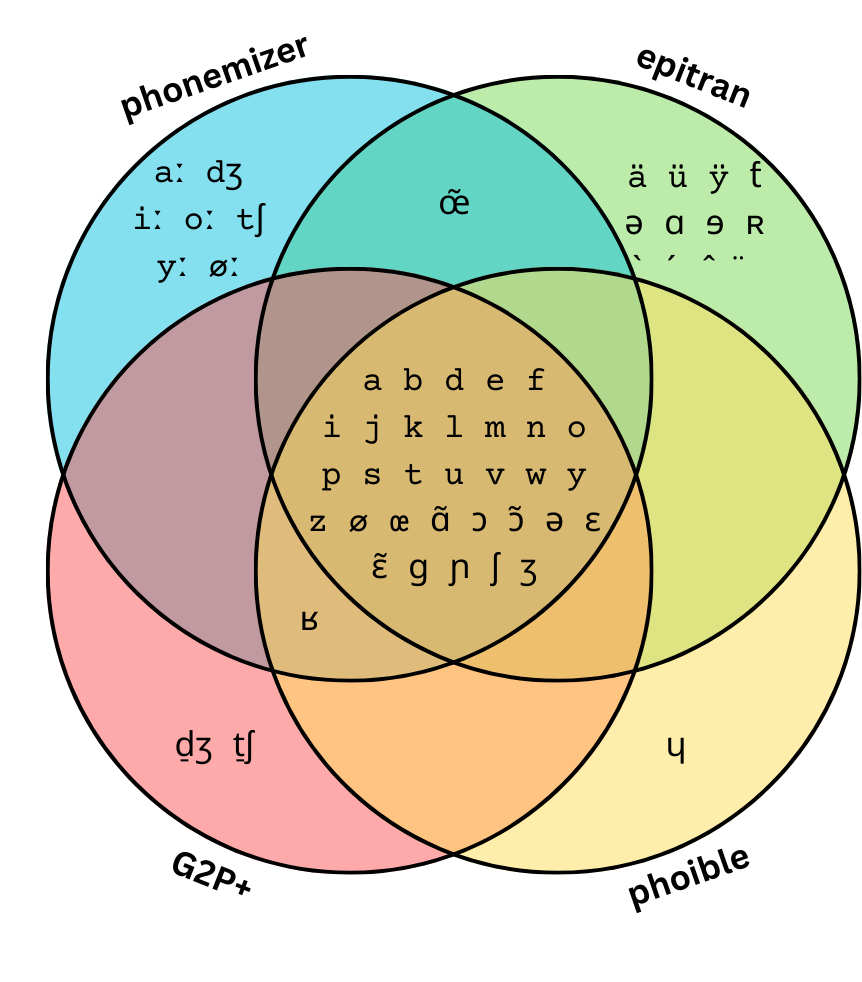
\includegraphics[width=0.5\linewidth]{13Resources/venn.png}
    \caption{Venn diagram of the inventories produced by \texttt{phonemizer}, \texttt{epitran} and \gpp compared to \phoible inventory \href{https://phoible.org/inventories/view/2269}{2269} for French.}
    \label{fig:13-venn}
\end{figure}

As G2P systems operate only from text, they may fail to capture accents and the variation found in natural speech\zeb{possibly forward ref to audio discussion here}. Nevertheless, G2P systems provide a useful method for producing phonemic transcriptions at scale, and were used to produce the transcriptions for LibriSpeech, VoxClamantis and IPAPACK. The fact that transcription errors may occur is often acknowledged as a limitation, but rarely are the outputs of different G2P systems compared to each other or to established inventories. For instance, \myemph{epitran} and \myemph{phonemizer} produce very different inventories for French, as demonstrated in \cref{fig:13-venn}. G2P provides a suitable method of converting the utterances in CHILDES to a phoneme-based representation and a new tool for G2P is introduced in the next section.

%In this chapter, existing statistical G2P tools are leveraged and their outputs are mapped to established \phoible inventories to produce consistent outputs. The resulting tool to is used to produce phonemic transcriptions for the utterances in the CHILDES database.

\section{\gpp}

I introduce \gpp as a tool for converting datasets from an orthographic representation to a phonemic representation. It operates either as a python library or as a command-line program; the user selects one of four backends and the language to use for conversion. Each backend supports a different set of languages as described in \cref{sec:13-backends}. The recommended backends for each of the languages in \ipachildes are given in \cref{sec:13-ipachildes}.

Each line of orthographic text is converted to phonemes, represented using IPA. Regardless of the backend selected, the representation is consistent, with phonemes separated by whitespace (for convenient tokenization, as discussed in \cref{sec:12-implementphoneme}). Word boundaries and utterance boundaries are represented using the unique symbols \texttt{WORD\_BOUNDARY}, and \texttt{UTT\_BOUNDARY}, respectively. 

The output representation is also consistent in terms of the set of phonemes types produced, using \emph{folding}, as described in \cref{sec:13-folding}. Without folding, each backend produces a different set of phonemes (as demonstrated in \cref{fig:13-venn}) which may not align with established phoneme inventories. The implemented folding maps not only ensure the output is consistent regardless of the backend chosen, but also makes it easy to leverage information in \phoible in analysis, as demonstrated in \cref{chapter:phonology}. Finally, qualitative evaluation of the tool is provided in \cref{sec:13-qualitative} and example usage is given in \cref{sec:13-usage}.

% The specific set of phonemes produced will be drawn from a vocabulary determined by the specific rules or pronunciation dictionaries created for the chosen backend and language. Since these tools are open-sourced, and since the exact \textbf{phoneme inventory} of languages are often up for debate, it is important to ensure that the phoneme inventory produced is consistent with established phoneme inventories for that language. This is accomplished using \emph{folding}, as discussed in \cref{sec:13-folding}.

\subsection{G2P backends}\label{sec:13-backends}

In order to support a wide variety of languages, wrappers are implemented over four backend G2P tools:

\paragraph{\myemph{phonemizer} \citep{Bernard2021}:} A python library for G2P in various languages based on \myemph{eSpeak}\footnote{For Japanese text written in Romanji, as is the case in CHILDES, phonemizer is used with the the Segments backend \citep{robert_forkel_2019_3549784}.}, an open-source speech synthesiser which supports over one hundred languages and accents \citep{Dunn2019}.

\paragraph{\myemph{epitran} \citep{Mortensen-et-al:2018}:} A python library that supports the automatic phonemization of text across many languages, accents and scripts, with a particular focus on low-resource languages. For the majority of the 92 languages supported\footnote{For English, Epitran uses the Flite Speech Synthesis System \citep{black2001flite} and for Simplified and Traditional Chinese it uses the CC-CEDict dictionary (\url{https://cc-cedict.org}).}, it uses greedily-interpreted grapheme-to-phoneme maps augmented with context-sensitive pre-processor and post-processor rewrite rules.

\paragraph{\myemph{pinyin-to-ipa} \citep{taubert_2024_pinyin-to-ipa_2024}:} A python library for converting Mandarin written in pinyin to IPA using a few contextual grapheme-to-phoneme maps. The phoneme inventory is based on the phonology of Mandarin as described by \cite{lin2007sounds} and \cite{duanmu2007phonology} and tone markers are attached to the vowel of the syllable, rather than the end of the syllable. The tool only converts individual pinyin syllables, so the wrapper first splits the input into syllables before using the tool to convert each syllable to IPA.

\paragraph{\myemph{pingyam}:} An open-sourced conversion chart\footnote{\href{https://github.com/kfcd/pingyam}{\myemph{github.com/kfcd/pingyam}}} between the various romanization systems of Cantonese (including IPA) based on data from the Open Cantonese Dictionary.\footnote{\href{https://www.kaifangcidian.com/han/yue/}{\myemph{www.kaifangcidian.com/han/yue/}}} The wrapper converts from the Jyutping system to IPA by first splitting the input text into syllables before using the table to convert each syllable to IPA. For consistency with \texttt{pinyin-to-ipa}, tone markers are moved to the vowel of each syllable. 

Although \texttt{pinyin-to-ipa} and \texttt{pingyam} only support one Chinese language each, they are included as backends because \texttt{epitran} and \texttt{phonemizer} have relatively poor G2P quality for these languages. This has prevented Chinese languages from being included in previous cross-lingual phonemic datasets \citep{ahn-chodroff-2022-voxcommunis} and has led to them being disregarded in cross-lingual analysis \citep{pimentel2020phonotactic}. The hope is that by including these backends, this gap is addressed. Tone markers are also combined with their preceding phoneme to create a unique token (e.g., \ttipa{a\tone{55}} is a single token, not two). Tone markers are thus treated as phonological features rather than as individual phonemes, similar to how diphthongs are unique phonemes. However, this decision is still debatable and does lead to a comparatively larger phonemic vocabulary, so an options is provided to disable this merging, as demonstrated in \cref{sec:13-usage}. 

\subsection{Phoneme inventory validation}\label{sec:13-folding}

In order to validate the set of phonemes produced by each choice of backend and language, I compare the output to the phoneme inventories for that language listed in \phoible, a database containing phoneme inventories extracted from source documents and tertiary databases for 2186 distinct languages \citep{phoible}. \phoible also contains typological data and phonological feature information for each phoneme, a useful resource for phonological analysis. As there are often multiple inventories in \phoible for each language, I choose the inventory that best matches the output phoneme of all backends that supports that language, according to the number of phoneme types, the number of consonants, the number of vowels and the number of diphthongs.

Once the best inventory has been found, a process called \emph{folding} is used to align the output phoneme set with the inventory and correct errors in the output. This is achieved using a manually-crafted look-up table (a \emph{folding map}) which is applied to the output of the G2P wrapper. These maps are primarily used to solve surface-level errors, instances where the G2P tool outputs a specific Unicode string for a specific phoneme but the inventory lists a different string. For example, the \myemph{phonemizer} backend with the \myemph{ja} language code (Japanese) outputs the tied characters \ttipa{\textroundcap{ts}} as one of the phonemes, but the Japanese inventory lists \ttipa{ts} instead. These errors can be solved with a simple one-to-one mapping, which only affects the surface form.

Besides these surface-level errors, other transcription errors can also be solved with folding maps in order to create a better alignment with a particular \phoible inventory, as detailed in \cref{tab:13-transcription-errors}. For example, the \texttt{epitran} backend for Serbian always outputs \ttipa{d Z} as two phonemes instead of the single phoneme \ttipa{dZ}, which can be solved with a single mapping. The many-to-one mappings and those that split or merge tokens may alter the number of output tokens or types. Since such a mapping will change the information-theoretic properties of the output, it is important that they are linguistically motivated and carefully implemented. 

\begin{table}[t]
    \centering
    \scriptsize
    \begin{tabular}{p{0.32\textwidth}p{0.26\textwidth}p{0.32\textwidth}}
    \toprule
        \textbf{Error type} & \textbf{Consequence} & \textbf{Example} \\
        \midrule
        \textbf{One-to-one:} The backend uses one symbol for a phoneme but the inventory lists a different symbol for that phoneme. & The one-to-one mapping does not change the number of types or tokens in the output. & \myemph{phonemizer} with language code \myemph{sv} (Swedish) outputs \ttipa{n} but the matching inventory uses \ttipa{\textsubbridge{n}}.\\
        \midrule
        \textbf{Many-to-one:} The backend produces two different phonemes that should only map to a single phoneme in the inventory. & The many-to-one mapping reduces the number of phoneme types. & \myemph{phonemizer} with language code \myemph{pt} (Portuguese) outputs both \ttipa{\*r} and \ttipa{r} but the matching inventory only lists \ttipa{K}.\\
        \midrule
        \textbf{Consonant merging:} The backend outputs two symbols for a consonant that should be written as a single phoneme. & The mapping merges the pair of consonants, reducing the number of phoneme tokens produced. & \myemph{epitran} with language code \myemph{srp-Latn} (Serbian) outputs the sequence \ttipa{d Z} but these are should be written as a single phoneme \ttipa{dZ}.\\
        \midrule
        \textbf{Vowel merging:} The backend outputs a pair of vowels as separate phonemes but they are typically analysed as a single diphthong. & The mapping merges the pair of vowels, reducing the number of phoneme tokens produced. & \myemph{pingyam} with language code \myemph{cantonese} outputs the sequence \ttipa{o u} but these are should be treated as a diphthong \ttipa{ou}.\\
        \midrule
        \textbf{Vowel splitting:} The backend outputs a diphthong that is not listed in the inventory and should be split into individual phonemes. & The mapping splits the pair of vowels, increasing the number of phoneme tokens produced. & \myemph{phonemizer} with language code \myemph{en-us} (North American English) outputs \ttipa{aIU} as a single phoneme but this should be \ttipa{aI U}.\\
        \midrule
        \textbf{Phoneme duplication:} The backend outputs duplicate phonemes to represent long vowels or consonants or because of an error. & The mapping replaces the pair of phonemes with just one, reducing the number of phoneme tokens. & \myemph{phonemizer} with language code \myemph{et} (Estonian) outputs \ttipa{d d} but should output the long consonant \ttipa{d:}.\\
        \midrule
        \textbf{Diacritic error:} The backend incorrectly outputs the diacritic as a separate symbol instead of attaching it to the phoneme. & The mapping may change the number of phoneme types or tokens. & \myemph{phonemizer} with language code \myemph{ko} (Korean) outputs the diacritic for aspiration as \ttipa{h} instead of \ttipa{\super{h}} so sequences \ttipa{kh} and \ttipa{ph} are mapped to \ttipa{k\super{h}} and \ttipa{p\super{h}}.\\
        \midrule
        \textbf{Orthographic error:} Due to an invalid symbol in the orthographic text, the backend outputs an incorrect phoneme. & The contextual mapping changes the frequency statistics for the resulting phoneme, possibly reducing the number of phoneme types. & \myemph{epitran} with language code \myemph{hun-Latn} (Hungarian) outputs \ttipa{\^o} when the orthographic letter \ttipa{\H{o}} is incorrectly written as \ttipa{\^o} and so the phoneme is mapped to \ttipa{\o:}.\\
        \bottomrule
    \end{tabular}
    \caption{A list of errors that can occur during G2P that can be fixed with a folding map.}
    \label{tab:13-transcription-errors}
\end{table}

In order to construct the folding map for each backend-language pair, I run \gpp on orthographic text for that language and compare the output set of phonemes $P_O$ to the phonemes in the closest inventory in \phoible $P_I$. Let the set of phonemes present in $P_O$ but not $P_I$ be the ``unknown phonemes'' $U_K$ where $U_K = P_O \setminus P_I $ and the set of phonemes present in $P_I$ but not $P_O$ be the ``unseen phonemes'' $U_S$ where $U_S = P_I \setminus P_O $. The folding map are then constructed as follows:
\begin{enumerate}
    \item Find pairs $(k,s) \in U_K \times U_S$ that differ according to an accent or diacritic and obviously represent the same phoneme (determined by ruling out alternatives or examining where $k$ is produced in the output). Create a one-to-one mapping $k:s$ for each such pair, e.g. \ttipa{t} : \ttipa{t\super{h}}.
    \item Find pairs $(k,s) \in U_K \times U_S$ that clearly represent the same phoneme (determined as above) but may use entirely different symbols, possibly due to an alternative transcription scheme. Create a one-to-one mapping for each pair, e.g. \ttipa{a} : \ttipa{\ae}.
    \item For remaining items $k \in U_K$, determine whether these result from one of the other errors in \cref{tab:13-transcription-errors}. Carefully examine instances where $k$ is produced in the output and create a suitable mapping $k : p$ for some $p \in P_I$ to solve the error (the mapping may need to be contextual or include several characters, e.g. \ttipa{\textrhookschwa} : \ttipa{@ \*r} or \ttipa{U O} : \ttipa{w O}). 
    \item For remaining items $s \in U_S$, determine whether these result from one of the other errors in \cref{tab:13-transcription-errors}. Carefully examine instances where $s$ should be produced in the output and create a suitable mapping $k : s$ for some $k \in P_O$ to solve the error (the mapping may need to be contextual or include several characters). 
    \item Examine the output for cases of \textbf{phoneme duplication} and other errors that may not contain phonemes in $U_K$ or $U_S$ but could still be solved with the phoneme map and create suitable mappings.
\end{enumerate}

The goal is for $U_K = \{\} = U_S$ or equivalently $P_I = P_O$, i.e the set of phonemes produced by the tool perfectly aligns with the phoneme inventory in \phoible. This is not always possible, often there are a few remaining phonemes in $U_K$ and/or $U_S$. This can occur when no obvious mappings could be found in steps 1--4 above. For example, the \texttt{epitran} backend for German does not produce the phoneme \ttipa{Z} (it is ``unseen'') and none of the unknown phonemes seem to be a good match. Another possibility is that the output set of phonemes $P_O$ may not align well with any of the \phoible phoneme inventories and so the closest match may not include some of the unknown phonemes $k \in U_K$ despite being valid phonemes for that language and listed in other inventories. For example, the \texttt{epitran} backend for German produce the phonemes \ttipa{x} and \ttipa{5} which are not listed in the matching inventory but are listed in other established inventories for German. In other cases, the unknown phonemes may come from loan words (e.g. \ttipa{ts} for ``pizza'' in Portuguese). Finally, there are some cases where the output considerably disagrees with all of the \phoible inventories but is a valid phonemic analysis of the language according to other sources.

\subsection{Usage}\label{sec:13-usage}

\gpp is a python library that can be used as an API or as a command-line tool in order to convert orthographic text to a phoneme-based representation. The tool allows the user to select the backend and language code to use for G2P with text provided through filepaths or standard input. Additional options include \verb|--keep_word_boundaries| to output a dedicated \texttt{WORD\_BOUNDARY} token between words and \verb|--uncorrected| to skip the folding process and output the phonemes exactly as produced by the backend tool. Each backend also supports individual options. For instance, \verb|--split-tones| outputs tones as individual tokens instead of merging them with the syllabic phoneme for our two Chinese language backends. 

\Zeb{Provide example outputs here?}


% For instance, the phonemic representation of ``what a conundrum!'' is:

% \vspace{-2mm}
% \begin{center}
% \texttt{\textipa{w 2 t} \textvisiblespace~\textipa{2} \textvisiblespace~\textipa{
% k @ n 2 n d \*r @ m} \textvisiblespace~}
% \end{center}
% \vspace{-1mm}

% \noindent
% One limitation of our phonemization tool is that `a' is not reduced to the shwah, `\textipa{@}', as it would be in continuous speech. We discuss the limitations of this phonemization process in \cref{sec:14-phonemeslimitations}. 


%\textbf{POSSIBLY MENTION THAT ENGLISH-US LANGUAGE CODE IS AN EXCEPTION BECAUSE WE HAVE TO MATCH BABYSLM}

% In \cref{app:13-endix:folding-dictionaries} I give the folding dictionary for each backend-language pair used in this thesis. I give the resulting phoneme inventory, describe the matching \phoible inventory and provide justification for any unknown or unseen phonemes.

\subsection{Qualitative analysis}\label{sec:13-qualitative}

%See \cref{sec:13-qualitative} for an example of using \gpp for French, using the \texttt{phonemizer} backend with a folding map to approach Phoible inventory \href{https://phoible.org/inventories/view/2269}{2269}.

\Cref{fig:13-venn} compares four sets of phonemes for French;
\begin{itemize}
\item the \phoible inventory for French\footnote{Phoible inventory \href{https://phoible.org/inventories/view/2269}{\myemph{2269}}},
\item the output of \myemph{phonemizer} on the French section of CHILDES,
\item the output of \myemph{epitran} on the French section of CHILDES,
\item the output of \gpp on the French section of CHILDES, when using \myemph{phonemizer} as a backend, and the crafted folding map.
\end{itemize}

The outputs of \myemph{phonemizer} and \myemph{epitran} both differ considerably from the \phoible inventory and from each other whereas the \gpp only fails to produce a single phoneme, \ttipa{\textturnh}, and produces two additional phonemes \ttipa{dZ} and \ttipa{tS}, which come from loanwords such as ``pizza'' and ``sandwich''. This high overlap allows analysis of data converted to phonemes using \gpp to easily lookup phoneme information in \phoible, such as phonological features, which would be more difficult if using the outputs of the other tools, which may not link to entries in \phoible.

\Zeb{Might need a bit more here.}

\section{\ipachildes}\label{sec:13-ipachildes}

To create \ipachildes, I first download all corpora in CHILDES that are monolingual and non-SLI to ensure each language partition contains naturalistic, monolingual speech. CHILDES has 48 languages but only 31 are supported by a backend in \gpp (either because the language is not supported, or because they have been transcribed using an irregular script). For languages supported by multiple backends, a sample transcription is produced using each backend and I carefully examine the output. The `best-fitting' backend (the one that produces a phonemic vocabulary closest to one of the inventories in \phoible) is selected and is the backend for which a folding map is produced, as described in \cref{sec:13-folding}. Having selected the best backend, \gpp is used to convert all orthographic utterances for each language to a phonemic representation, producing a CSV containing the original representation, the phonemic representation as well as additional data stored in CHILDES (such as target child age, morpheme count, part of speech information, and the IDs of each utterance, transcript, corpus and collection). 

The resulting dataset contains 45 million words of monolingual child-centred speech for 31 languages. The data is sorted by child age in order to support curriculum learning experiments, such as in the work of \citet{huebner-etal-2021-babyberta}, and an `is\_child' feature is provided to allow for filtering child or adult utterances.

An illustration of the dataset is given in \cref{fig:13-overview} and a description of each language section is given in \cref{tab:13-phonemized-childes-sections}, detailing the matching \phoible inventory and CHILDES section for each language. Note that English is divided into British English (EnglishUK) and North American English (EnglishNA) to mirror the split present in CHILDES and Portuguese is also split into European and Brazilian varieties, following previous work \citep{caines2019cross}. For these splits, different \texttt{phonemizer} accents are used. Data is not uniformly distributed across languages. EnglishNA is the most represented, with close to 10 million words, and Farsi is the least represented, with only 43 thousand words. Limitations of the dataset are discussed in \cref{sec:13-limitations}.

%due to the phonological differences between Brazilian and Portugal Portuguese, the availability of language codes to phonemize the two, and the fact that the corpora are distinct within CHILDES.
\begin{table}[t!]
    \centering
    \footnotesize
    \begin{tabular}{lllccc}
        \toprule
        \textbf{Language} & \textbf{CHILDES Collection} & \textbf{Backend} & \textbf{Phoible} & \textbf{Words} & \textbf{\% Child} \\ 
        \midrule
        EnglishNA & \href{https://childes.talkbank.org/access/Eng-NA}{EnglishNA} (49) & \texttt{phonemizer} & \href{https://phoible.org/inventories/view/2175}{2175} & 9,993,744 & 36 \\
        EnglishUK & \href{https://childes.talkbank.org/access/Eng-UK}{EnglishUK} (16) & \texttt{phonemizer} & \href{https://phoible.org/inventories/view/2252}{2252} & 7,147,541 & 39 \\
        German & \href{https://childes.talkbank.org/access/German}{German} (10) & \texttt{epitran} & \href{https://phoible.org/inventories/view/2398}{2398} & 5,825,166 & 44 \\
        Japanese & \href{https://childes.talkbank.org/access/Japanese}{Japanese} (11) & \texttt{phonemizer} & \href{https://phoible.org/inventories/view/2196}{2196} & 2,970,674 & 44 \\
        Indonesian & \href{https://childes.talkbank.org/access/EastAsian}{EastAsian/Indonesian} (1) & \texttt{epitran} & \href{https://phoible.org/inventories/view/1690}{1690} & 2,347,642 & 34 \\
        French & \href{https://childes.talkbank.org/access/French}{French} (15) & \texttt{phonemizer} & \href{https://phoible.org/inventories/view/2269}{2269} & 2,973,318 & 40 \\
        Spanish & \href{https://childes.talkbank.org/access/Spanish}{Spanish} (18) & \texttt{epitran} & \href{https://phoible.org/inventories/view/164}{164} & 2,183,992 & 46 \\
        Mandarin & \href{https://childes.talkbank.org/access/Chinese}{Chinese/Mandarin} (16) & \texttt{pinyin\_to\_ipa} & \href{https://phoible.org/inventories/view/2457}{2457} & 2,264,518 & 39 \\
        Dutch & \href{https://childes.talkbank.org/access/DutchAfrikaans}{DutchAfricaans/Dutch} (5) & \texttt{phonemizer} & \href{https://phoible.org/inventories/view/2405}{2405} & 1,475,174 & 35 \\
        Polish & \href{https://childes.talkbank.org/access/Slavic}{Slavic/Polish} (2) & \texttt{phonemizer} & \href{https://phoible.org/inventories/view/1046}{1046} & 1,042,841 & 63 \\
        Serbian & \href{https://childes.talkbank.org/access/Slavic}{Slavic/Serbian} (1) & \texttt{epitran} & \href{https://phoible.org/inventories/view/2499}{2499} & 1,052,337 & 29 \\
        Estonian & \href{https://childes.talkbank.org/access/Other}{Other/Estonian} (9) & \texttt{phonemizer} & \href{https://phoible.org/inventories/view/2181}{2181} & 843,189 & 45 \\
        Welsh & \href{https://childes.talkbank.org/access/Celtic}{Celtic/Welsh} (2) & \texttt{phonemizer} & \href{https://phoible.org/inventories/view/2406}{2406} & 666,350 & 69 \\
        Cantonese & \href{https://childes.talkbank.org/access/Chinese}{Chinese/Cantonese} (2) & \texttt{pingyam} & \href{https://phoible.org/inventories/view/2309}{2309} & 777,997 & 34 \\
        Swedish & \href{https://childes.talkbank.org/access/Scandinavian}{Scandinavian/Swedish} (3) & \texttt{phonemizer} & \href{https://phoible.org/inventories/view/1150}{1150} & 581,451 & 45 \\
        PortuguesePt & \href{https://childes.talkbank.org/access/Romance}{Romance/Portuguese} (4) & \texttt{phonemizer} & \href{https://phoible.org/inventories/view/2206}{2206} & 499,522 & 39 \\
        Korean & \href{https://childes.talkbank.org/access/EastAsian}{EastAsian/Korean} (3) & \texttt{phonemizer} & \href{https://phoible.org/inventories/view/423}{423} & 263,030 & 37 \\
        Italian & \href{https://childes.talkbank.org/access/Romance}{Romance/Italian} (5) & \texttt{phonemizer} & \href{https://phoible.org/inventories/view/1145}{1145} & 352,861 & 39 \\
        Croatian & \href{https://childes.talkbank.org/access/Slavic}{Slavic/Croatian} (1) & \texttt{epitran} & \href{https://phoible.org/inventories/view/1139}{1139} & 305,112 & 39 \\
        Catalan & \href{https://childes.talkbank.org/access/Romance}{Romance/Catalan} (6) & \texttt{phonemizer} & \href{https://phoible.org/inventories/view/2555}{2555} & 319,726 & 36 \\
        Icelandic & \href{https://childes.talkbank.org/access/Scandinavian}{Scandinavian/Icelandic} (2) & \texttt{phonemizer} & \href{https://phoible.org/inventories/view/2568}{2568} & 279,939 & 35 \\
        Basque & \href{https://childes.talkbank.org/access/Other}{Other/Basque} (2) & \texttt{phonemizer} & \href{https://phoible.org/inventories/view/2161}{2161} & 230,500 & 49 \\
        Hungarian & \href{https://childes.talkbank.org/access/Other}{Other/Hungarian} (3) & \texttt{epitran} & \href{https://phoible.org/inventories/view/2191}{2191} & 237,062 & 48 \\
        Danish & \href{https://childes.talkbank.org/access/Scandinavian}{Scandinavian/Danish} (1) & \texttt{phonemizer} & \href{https://phoible.org/inventories/view/2265}{2265} & 275,170 & 42 \\
        Norwegian & \href{https://childes.talkbank.org/access/Scandinavian}{Scandinavian/Norwegian} (2) & \texttt{phonemizer} & \href{https://phoible.org/inventories/view/499}{499} & 227,856 & 43 \\
        PortugueseBr & \href{https://childes.talkbank.org/access/Romance}{Romance/Portuguese} (2) & \texttt{phonemizer} & \href{https://phoible.org/inventories/view/2207}{2207} & 174,845 & 44 \\
        Romanian & \href{https://childes.talkbank.org/access/Romance}{Romanian} (3) & \texttt{phonemizer} & \href{https://phoible.org/inventories/view/2443}{2443} & 152,465 & 43 \\
        Turkish & \href{https://childes.talkbank.org/access/Other}{Other/Turkish} (2) & \texttt{phonemizer} & \href{https://phoible.org/inventories/view/2217}{2217} & 79,404 & 51 \\
        Irish & \href{https://childes.talkbank.org/access/Celtic}{Celtic/Irish} (2) & \texttt{phonemizer} & \href{https://phoible.org/inventories/view/2521}{2521} & 105,867 & 34 \\
        Quechua & \href{https://childes.talkbank.org/access/Other}{Other/Quechua} (2) & \texttt{phonemizer} & \href{https://phoible.org/inventories/view/104}{104} & 46,848 & 40 \\
        Farsi & \href{https://childes.talkbank.org/access/Other}{Other/Farsi} (2) & \texttt{phonemizer} & \href{https://phoible.org/inventories/view/516}{516} & 43,432 & 40 \\
        \bottomrule
    \end{tabular}
    \caption{A breakdown of each language available in \ipachildes. The bracketed number in the \textbf{CHILDES Collection} column refers to the number of corpora downloaded from that collection. The \textbf{Backend} refers to the \gpp backend  used to convert utterances for that language to phonemes. \textbf{Phoible} links to the \phoible inventory used for that language in folding. The \textbf{Words} columns refer to the number of words in each subset and \textbf{\% Child} refers to the percentage of the data that is child-produced (rather than adult-produced).}
    \label{tab:13-phonemized-childes-sections}
\end{table}

\ipachildes addresses several limitations of past datasets, as the first large multilingual corpus of child-centred phonemic speech. \Cref{chapter:modelling} and \cref{chapter:phonology} demonstrate how this data can be used to train phoneme LMs, but \ipachildes could also support information-theoretic studies of language processing and acquisition, which have previously based their calculations on word types \citep{piantadosi2011word, dautriche2017words, pimentel2020phonotactic} or orthographic text \citep{mahowald2013info, dautriche2017wordform, futrell2020lossy}, often citing a lack of phonemic data as a limiting factor. The child-centred domain of \ipachildes could also be beneficial for studying the `Goldilocks' hypothesis \citep{kidd2014goldilocks} and the properties of `Parentese' \citep{ramirez2017look}. An example experiment investigating the later is provided in \cref{app:parentese}, where the average information of utterances directed to children aged 0--6 across 10 languages is computed, revealing a general trend of increasing informative content.

\section{Limitations}\label{sec:13-limitations}

\gpp is as an open-sourced G2P tool for converting orthographic text to a phoneme-based representation, improving on previous tools by ensuring output phoneme sets are consistent with inventories found in the \phoible database. It is used to create \ipachildes, the first large multilingual corpus of child-centred speech represented using phonemes. Although these provide useful resources for phonological experimentation, there are some limitations, which are considered here.

\paragraph{Phonemes as a representation of speech:} While phonemic data more closely represents how words are pronounced compared to orthographic text (the degree of this difference varies between languages), phonemes are still abstract symbolic units which do not contain many of the detailed and continuous features of speech, such as prosody. They also abstract away from phones, which are detailed realizations of phonemes, representing the physical sound produced rather than a language-specific meaningful unit. Nevertheless, phonemes still provide a useful unit of analysis and are necessary for certain linguistic theories and information-theoretic calculations. While phones could offer another useful representation, they are even harder to source than phonemes.

\paragraph{G2P conversion inaccuracies:} Although \gpp uses folding maps to improve the output of the backend tools, these backends still vary in quality across the supported languages. When converting each language in CHILDES, the most appropriate backend for each language is selected (and noting the poor quality of other tools for Chinese languages, two backends are added to support G2P for Mandarin and Cantonese), but the output quality may still vary. Many of the G2P tools for certain languages convert words individually, which may not capture vowel reduction, allophonic variation or other differences found in natural speech. A single accent is also utilised for each language, losing inter-speaker variability. The \myemph{phonemizer} backend does support multiple accents for certain languages (here we a different accent is used for EnglishNA and EnglishUK) and future work could try to maintain accent differences during G2P, but this would require speaker information or audio, as was done during the creation of Audio BNC \citep{coleman2012audio}. Finally, G2P methods may not produce correct transcriptions for the child-produced utterances in CHILDES, which are often corrected by the transcriber, especially for young infants. Initially I intended to distribute \ipachildes without child-produced utterances (and in this thesis models are only trained models with the child-directed utterances) but as they might be useful in future research, I instead note this limitation.

\paragraph{Phoible inventories:} Although the \phoible database collects established phonemic inventories and provides distinctive feature vectors, there are still often multiple phoneme inventories for a single language. This the exact phonemic inventory for a particular language is still a matter of debate among expert phonologists. When creating folding maps, the `best-fitting' inventory to map to is chosen, as detailed in \cref{tab:13-phonemized-childes-sections}, but these inventories may not be exact.

\paragraph{Languages:} Although \ipachildes is multilingual, there are still limitations in terms of language coverage. The languages are predominantly European and Asian, with no languages indigenous to the Americas, Australia or Africa. English is also still the dominant language of the dataset and the Farsi section is very small, only containing 43 thousand words. The creation of this dataset was limited by the languages available in CHILDES. The languages in CHILDES not able to be converted were Greek, Arabic, Hebrew, Thai, Georgian, Tamil, Taiwanese, Jamaican, Sesotho, Berber, Cree and Slovenian and Russian due to missing G2P backends or unsupported scripts.

% \paragraph{Phoneme LMs:} We train phoneme LMs on 11 languages from \ipachildes but the specific architecture we use is based on our scaling experiment for the EnglishNA model. Although we do not directly compare these LMs, we note the possibility that other parameters may have better suited the non-English languages. We were only able to conduct the scaling experiments for English due to the lack of phonological benchmarks for other languages but we hope that the release of \ipachildes facilitates further work in multilingual phonological evaluation of phoneme LMs.


\section{Summary}

This chapter introduces \gpp and \ipachildes, two new resources for phonological research. \gpp improves open-source G2P tools by ensuring phonemic vocabularies align with the established inventories in the \phoible database. Using this tool, \ipachildes is created by converting the orthographic transcriptions in CHILDES into phonemic representations, resulting in a large corpus of child-centred spontaneous speech across 31 languages.

\gpp and \ipachildes are designed to enable a wide range of future studies in linguistics and NLP, particularly in phonological acquisition, cross-linguistic analysis, and speech processing. In this thesis, \gpp is first used in \cref{chapter:modelling} to convert the BabyLM dataset and evaluation benchmarks to phonemes to facilitate a comparison of input representations, then \ipachildes is used in \cref{chapter:phonology} to explore the distributed phonological representations learned by phoneme LMs. 


%Our results indicate the utility of phoneme LMs for emergent phonology and we anticipate many other future studies that our resources could facilitate across linguistics and NLP.

%We intend for this dataset to facilitate future work in experimental phonetics, where prior work based calculations on word types or orthographic text, future calculations could use the phonemic word tokens in our dataset to provide better frequency statistics and more closely resemble speech. We also use our dataset to extend recent work exploring phoneme-based pre-training of language models to the multilingual setting. %By linking to \phoible, we show that these models can be probed for phonological features, finding that while certain features (e.g. \texttt{consonantal}) seem to play a role in distributed phonetics, others (e.g. \texttt{delayedRelease}) do not. Finally, we use the BabySLM metric to demonstrate the model sizes required to learn phonology and syntax with phoneme LMs.


% \paragraph{Phoneme LMs:} We train phoneme LMs on 11 languages from \ipachildes but the specific architecture we use is based on our scaling experiment for the EnglishNA model. Although we do not directly compare these LMs, we note the possibility that other parameters may have better suited the non-English languages. We were only able to conduct the scaling experiments for English due to the lack of phonological benchmarks for other languages but we hope that the release of \ipachildes facilitates further work in multilingual phonological evaluation of phoneme LMs.






% \subsection{Limitations and advantages of phonemic transcriptions}
% \label{sec:14-phonemeslimitations}

% One difficulty in training models from ecological long-form child-centred audio is the lack of corpora available. Papers reporting research on day-long recordings tend not to release the raw data due to privacy concerns (e.g.\ \citet{bergelson-etal-2023,leon-cristia-2024}).
% Our method allows us to convert text (which is much more readily available) into a speech representation (phoneme streams), meaning that we could quickly prepare a corpus of 100 million words. 

% There are also limitations in our transcription generation process. The fact that phonemes are an abstraction of speech means that we lose key information contained in speech such as prosody, stress and allophonic variation. Using a single accent to generate our phonemes, we also lose inter-speaker variability. Children also learn from non-linguistic cues, multi-modal input and interaction. If anything, it is a striking result that a model trained only on a set of 51 discrete symbols is able to demonstrate grammatical knowledge and perform competitively at downstream linguistic tasks. 

% %[Effect of noise: only 51 symbols to choose from for phoneme data, so each carries less information, so an difference in one token would be harder for the language model to get right compared to 115 characters (possibly). With subwords, way more possibility for distinguishing. Maybe move this up to results and do detailed analysis of some examples.]
